\part{Introduction}

    \chapter{Overview}

        This project is focused on marrying new technological trends, like smartphones and wearable devices, and medical data collection so that medical professionals have the capability to capture large amounts of data. This data can then be used to further inform the medical professional's decisions. In years past, in order to capture data from a patient, the patient would often have to come into a testing center or a professional had to go to the patient; this is costly in both time and money, so this project seeks to eliminate or lessen some of these barriers. 

        By using sensors provided in smartphones and wearables, this project seeks to monitor and quantify certain activities like walking and sleeping in day to day life.

    \chapter{Motivation}

        \section{Pulmonary Disease and Heart Failure}

            Where such monitoring as described above can be most useful is when concerned with diseases like chronic obstructive pulmonary disease and heart failure. Both these diseases affects a person's ability to engage in physical activity and both tend affect similar groups of people [CIT]. By monitoring a person's, who is afflicted with either of these diseases, activity and sleep records, medical professional may be able to track a patient's condition on a frequent basis. This can allow for early prevention or intervention.

            Chronic Obstructive Pulmonary Disease (COPD) is the name for a set of lung conditions that are the source of breathing difficulties. COPD is a relatively common disease for middle-aged or older adults. According to the British Lung Foundation, around 4.5\% of adults aged 45 and older are diagnosed with this condition [CIT]. Often times the affected does not realize that they have the disease, but their breathing problems get gradually worse. The disease cannot be cured or reversed, but treatment may keep it under control so that it does not impact their daily life. Part of this treatment may be what is known as 'pulmonary rehabilitation', a specialised programme of exercise. [CIT]

            Heart failure is a condition where the heart is unable to pump blood around the body properly, this usually occurs because the heart is too stiff or weak. According to the British Heart Foundation, around half a million people in the UK have been diagnosed with heart failure [CIT]. There are four classes or stages of heart failure, with a higher class signifying higher severity. 

        \section{Six Minute Walk Test}

            As mentioned above, there are a number of diseases like COPD or heart failure that impact a patient's ability to engage in physical activity. These diseases have no cure and generally tend to get worse with time. In many cases, the degree of physical activity that the patient can undergo can indicate the severity of the disease [CIT]. This fact is utilized in the application of the Six Minute Walk Test (6MWT).

            The Six Minute Walk Test (6MWT) is a standardized test of functional exercise that involves walking along a flat, straight course for six minutes. The test is self paced and there are no requirements regarding speed or breaks. The 6MWT is often used to track therapy progress and has been proven to be sensitive to common therapies [CIT]. Typically the variable that is measured is the distance walked in the six minutes. However, oxyhaemoglobin saturation and heart rate can be measured too. 

            The 6MWT is often used as part of tracking a patient's recovery or condition for diseases like those listed above. [CIT]

        \section{Smartphones and Wearables}

            In recent years the increasing penetration of the smartphone has been rapid and widespread. According to the Deloitte Mobile Consumer Survey 2016 [CIT], 91\% of people in the UK aged 18-44 own a smartphone. Additionally, Statista reports that in 2015 50\% of those surveyed aged 55-64 owned a smartphone and 18\% aged 65+ owned a smartphone [CIT]. Clearly, the adoption of the smartphone is reaching saturation among the general populace, particularly the younger generations.

            Parallel to the increasing adoption of smartphones is the increasing capabilities of such devices. For example, the BLU Diamond M Android Smartphone which is available for \textsterling39.99 on AmazonUK [CIT]. This phone has a 1.3 GHz quad-core processor and 512MB RAM [CIT]. Compare this to flagship devices from prior years, for example, the Samsung Galaxy S3 released in May 2012 at a cost of \$599 at launch. This device had a 1.4 Ghz quad-core processor and 1GB RAM [CIT]. The cost to performance ratio for such devices has dropped dramatically in recent years.

            Another important factor to consider is the availability of sensors in these devices. Even such low end devices as the BLU Diamond M has a built in accelerometer and proximity sensor. [CIT] Higher end devices will have additional sensors such as gyroscope, barometer, or a magnetometer. This availability of sensors across the board allows for a unique opportunity for widespread, remote data collection. 

            For example, the 6MWT described above can be performed by the patient using a certified application that counts the steps automatically. This is far easily and less costly than having the patient attend a testing center to record these results.

            In addition, wearables have taken off in the last few years with big players like Apple introducing the Apple Watch in 2015 and Google debuting Android Wear in 2014. Along with these more general purpose devices are more niche devices like those developed by FitBit or Jawbone that are aimed at fitness enthusiasts. These new devices are packed with sensors like smartphones noted above. This provides another avenue for easy day-to-day data collection.

    \chapter{Objectives}

        \section{Step Counter}

            In order to track 6MWT performance, a generalized step counting algorithm must be available. More modern smartphones often incorporate step counters on device, but older devices still lack this functionality. Applications like Google Fit aim to do a similar thing, however, the mechanism of these applications are unknown. In addition, there are wearable devices such as a Fitbit or Jawbone that incorporate step counters based off the accelerometers. Again, the mechanism of such devices are not published and extracting data from such services is tricky at best. Due to the opaque nature of such devices and software, they cannot be easily tuned for medical use.

            In order to reach the maximum number of potential users, the step counter algorithm shall target smartphone devices as the penetration of these devices is much higher. Also, there are only two platforms to target in order to capture the majority of the market (iOS and Android). This algorithm shall only use the accelerometer signal for its algorithm, again, to maximize the number of potential users.

            As accelerometer signals are often very noisy, this algorithm must be robust to noise and capable accuracies sufficiently high to enable meaningful analysis of the results. Additionally, this algorithm should be computationally efficient so as to run in realtime on a smartphone device.

            The performance of this algorithm will be validated against the ground truth data collected by a proprietary device, described in Section [SECTION]. The metric of interest is the total number of steps over a given time period. This report shall not discuss the false positive rate, the rate at which the algorithm identifies a step when there isn't one, or the false negative rate, the rate at which the algorithm does not identify a step when there is one, of the algorithm.

        \section{Sleep Detection}

            The other component necessary to the project is an accurate sleep detector. While it is unlikely that accelerometer driven sleep detectors will reach the classification accuracy achieved by the gold standard, polysomnography, they represent a very accessible alternative that can provide a rough estimate of sleep onset and duration. Polysomnography is a study that is done on a patient, typically to diagnose sleep disorders. The patient undergoing polysomnography has their brain waves, oxygen levels in the blood, heart rate, breathing, eye movement, and leg movement recorded. The data is later analysed by a trained professional, who produces a dataset relating how the patient transitions between sleep stages (deep sleep, REM, awake) during the night.

            The feasibility of such algorithms has been demonstrated with consumer products such as those sold by Fitbit.

            The algorithm and methodology behind these commercial trackers are unknown and Fitbit keeps their data under lock and key, users cannot access the hard data inside the device. So to overcome this limitation, a sleep detection algorithm will be written that operates on a wrist-mounted accelerometer, such as in a device like an Apple Watch. A wearable device was chosen for this aspect of the project as it can be easily fastened to the user during sleep, unlike a smartphone which cannot be guaranteed to be in the same place the entire night.

            This algorithm seeks to discern the sleep onset time, the time at which the user falls asleep, and wakefulness onset time, the time at which the user wakes up, using the accelerometer signal provided by a wrist mounted smart device such as the Apple Watch.

            In order to develop and validate the algorithm, a database produced by the Embedded Sensing Systems Group at TU Darmstadt was used [CIT]. This database contains both the actigraphy traces and annotated polysomnography for 42 sleep lab patients.

            The performance will also be tested against similar devices such as a Fitbit device [CIT] or the Sleep As Android application [CIT]. 


    \chapter{Literature Review}


        \section{Step Counting}

            \subsection{Mechanics of Walking}

                The act of walking is detailed in Naqvi, et. al. [CIT] and is as follows:

                \begin{enumerate}
                    \item At the beginning of the step, the planted foot is pushed backwards into the floor.
                    \item Static friction opposes this force. This provides the driving force forward.
                    \item At the end of the step the stepping foot is placed on the floor and pushes forward into the floor.
                    \item Again, static friction opposes this force, giving rise to a backwards force.
                \end{enumerate}

                An example of raw accelerometer data of walking is shown below in Figure \ref{img_accel_ex}. It should be quite clear that the act of walking gives rise to periodic activity with a period corresponding to a single step. 

                \begin{figure}[h]
                    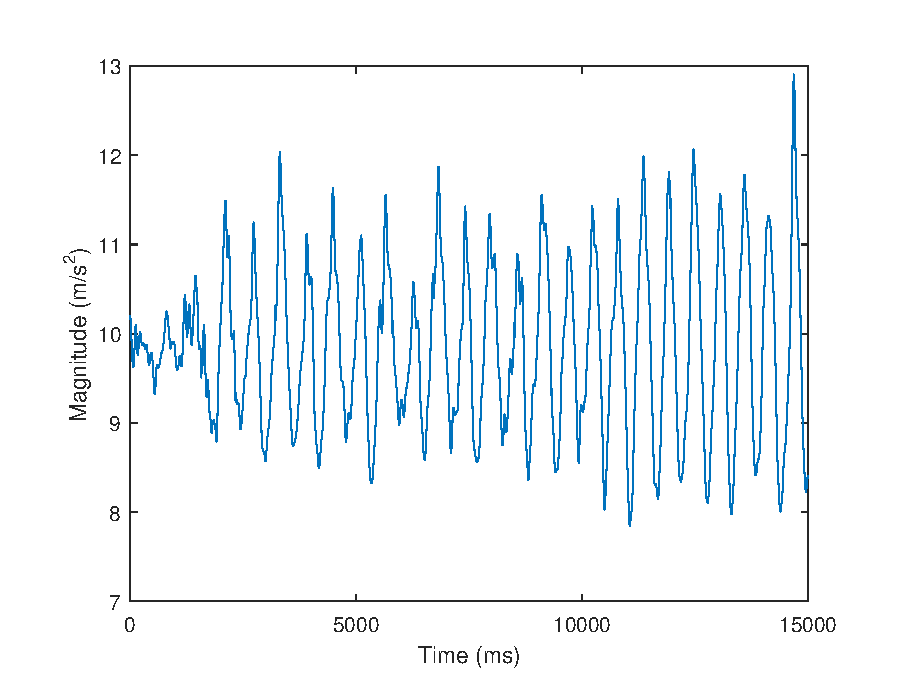
\includegraphics[width=\textwidth]{Images/accel_signal.eps}
                    \centering
                    \caption{Example of an accelerometer signal recorded during a period of walking.}
                    \label{img_accel_ex}
                \end{figure}

            \subsection{Previous Attempts}

                There have been a number of attempts to do step counting with purely an accelerometer signal, so the literature is fairly rich from this aspect. 

                In Navqi, et. al. [CIT] a relationship between walking speed and the magnitude of the accelerometer is derived and used in devising a algorithm that is based on thresholding the mangitude of the signal. The algorithm is then tested on 5 samples ranging from 16-44 steps long and achieves an average accuracy of 96.6\%. The collection protocol is not noted besides the fact that the the signal is collected by a device fixed at the center of mass of the subject. 

                In Brajdic and Harde [CIT], the authors test a multitude of types of algorithms for both walk detection and step counting. This paper is only interested in step counting, so walk detection algorithms will be ignored. The authors note that many algorithms involve some sort of thresholding some property of the signal, especially when the sensor is placed at the foot. However, it is mentioned that choosing an optimal threshold is difficult for different users, surfaces, or shoes. Other algorithms use peak detection or zero-mean crossings to count steps. In the frequency domain, they note that some algorithms use the inherent periods of walking to search for periods of walking and can hence calculate fractional steps. This is done either via the Short Term Fourier Transform or Wavelet Transforms. An equivalent option to these transforms is to use the autocorrelation in the time domain, large magnitudes indicate high periodic activity at those lags. All of these algorithms suffer from the problem that they will be triggered by any movement with a similar periodicity to walking. A more complex algorithm involves non-linear template matching with dynamic time warping. A generic template can be generated offline and then correlated in real time with the signal. 

                The authors also explored machine learning based techniques, with commonly used features like: mean, variance, energy, entropy, correlation between axes, and FFT coefficients. They note previous attempts use classifiers like: neural networks, Gaussian mixture models, or support vector machines. Sometimes, non-parametric classification like k-nearest neighbors was used. The authors note Hidden Markov Models are used often, and fit the problem well as the input to these models are a sequence of temporal values.

                From this list of techniques, the authors chose 9 to evaluate. These 9 were: windowed peak detection, mean crossing counts, normalized autocorrleation, dynamic time warping, short term fourier transform, continuous wavelet transform, discrete wavelet transform, hidden markov model, and k-means clustering. 

                In order to evaluate all of these algorithms, the authors collected 130 data recordings from 27 subjects with a Galaxy Nexus GT-I9250 across a variety of scenarios: in hand, in a pocket, in a back pocket, or in a handbag. A video recording was taken of each recording for later validation.

                With the data recordings and these algorithms, the authors concluded that the windowed peak detection, hidden markov model, and continuous wavelet transform methods worked the best. With a median error of 1.3\% for each. Note that this was done with 80 of the 130 data recordings that had 'reliable ground truth step counts'. The authors also note that the placement of the phone had little effect on the step counting performance. 

                In Palshikar [CIT], the author describes a methodology of peak detection in time-series. The author describes the general flow of the the method in which each point in the series is scored on how peaky it is and then search for local peaks using the standard deviation and mean of the signal. THe author provides a few characterizations of the scoring function $S(x_i)$. This methodology forms the basis for part of the algorithm described later.

        \section{Sleep Detection}

            The literature is much less rich for sleep detection with a wrist-mounted accelerometer as wearable devices are a relatively new invention. 

            In Borazio, et. al. [CIT] the authors tried to solve this exact problem. The authors built a custom device to be worn on the wrist with an accelerometer that records at 100Hz. They collected a dataset containing 409 hours of sleep lab data, meaning that each data recording comprises of a night's sleep from one patient. The patient underwent polysomnography the same night to provide a ground truth. The authors proposed a simple algorithm that thresholds the acceleration signal based on the standard deviation of the magnitude. If the last 100 points (1 second of recording) exceeds a threshold, then the user is marked as not sleeping. Then the authors ensure a minimum length for intervals that the user is not sleeping. The authors compared their method against the well known Oakley and Cole algorithms that use activity counts to determine wakefulness, as well as against the ground truth polysomnography. 

            The results show that the novel approach marginally outperforms the Oakley and Cole algorithms (79.83\% vs 74.94\% and 73.75\% respectively). The author notes that where all the algorithms fail is when the patient is not asleep but simply not moving. The dataset collected has been made publically available and will be used later in the paper. 

            In van Hees, et. al. [CIT], the authors attempt to classify sleep using the arm-angle of the patient. The author states that sleep is characterized by a period of low frequency of changes in arm-angle. The methodology consists of calculating the arm angle using rolling medians of the x, y, and z components of acceleration and then assessing changes in arm angle between 5 second epochs. If there was no change larger than $5^{\circ}$ in 5 minutes, then these were classified as sustained inactivity. The accelerometer data was collected along with a self reported sleep log of onset and offset. The author notes that overall there was moderate agreement between the accelerometer and self reported sleep duration.